\chapter{Implementation}
\label{ch:impl}

The system is implemented in Python 3.12 as four packages (\code{honeypot}, \code{pipeline},
\code{dashboard}, \code{simulator}) and deployed as five containers. Table~\ref{tab:loc}
summarises its size.

\begin{table}[H]
\centering
\begin{tabular}{@{}lrrr@{}}
\toprule
\textbf{Package} & \textbf{Source lines} & \textbf{Test lines} & \textbf{Tests} \\
\midrule
\code{honeypot} & 3{,}344 & 444 & 69 \\
\code{pipeline} & 375 & 191 & 12 \\
\code{dashboard} (+514 lines of templates, CSS, JS) & 328 & 112 & 20 \\
\code{simulator} & 879 & 101 & 10 \\
\midrule
Total & 4{,}926 & 848 & 111 \\
\bottomrule
\end{tabular}
\caption{Implementation size.}
\label{tab:loc}
\end{table}

\section{The Honeypot}

\subsection{SSH Server and Login Policy}

The server is built on AsyncSSH~\cite{asyncssh}. It advertises the version string of the
OpenSSH build that Ubuntu~22.04 ships,
\code{OpenSSH\_8.9p1\ Ubuntu-3ubuntu0.4}, and presents
both RSA and Ed25519 host keys. The keys are generated once and kept in a volume, so the
server's fingerprint is stable across restarts; a changing fingerprint is a honeypot tell.

Accepting every password on the first try is another well-known tell. For each source IP the
server therefore draws a threshold $N \sim U\{1,\dots,3\}$ and accepts the $N$-th attempt. Every
attempt (username, password, attempt number, outcome) becomes a \code{login\_attempt} event.

\subsection{Fake Filesystem}
\label{sec:fs}

Each session receives its own \code{FakeFileSystem}, an in-memory tree of nodes with
permissions, owners and timestamps. It is generated procedurally from a seed and discarded at
disconnect. It reproduces an Ubuntu~22.04 web/database server:
\begin{itemize}
  \item a standard root hierarchy and \code{/etc} (\code{passwd}, \code{shadow}, \code{group},
    \code{os-release}, \code{sshd\_config}, \code{crontab}, \code{nginx}, \code{mysql});
  \item \code{/proc} entries (\code{cpuinfo}, \code{meminfo}, \code{version}; \code{uptime} is computed live);
  \item lived-in content: a 60-line \code{auth.log} of failed logins, \code{syslog}, a nightly
    backup script and its log, \code{.bash\_history} for three users, binaries of realistic
    sizes in \code{/usr/bin}, and timestamps scattered over the past year;
  \item Unix permissions: a non-root user cannot read \code{/etc/shadow} or list \code{/root}.
\end{itemize}

\act{fake} calls \code{plant\_decoys()}, which idempotently adds honeytoken files and extends
\code{.bash\_history} with commands that point to them:
\begin{itemize}
  \item \code{/root/backup\_credentials.txt} and \code{/root/.my.cnf};
  \item \code{/home/deploy/.env};
  \item \code{/var/www/html/wp-config.php}.
\end{itemize}
To keep the repository free of anything resembling a real secret, every decoy value is a
visible placeholder such as \code{<decoy:mysql-root>}. The experiments measure \emph{whether}
attackers read decoys, which does not depend on how convincing the values look.

\subsection{Shell Emulator}

\code{Shell} parses each input line into statements separated by \code{;}, \code{\&\&},
\code{||} and \code{\&}. Exit status is tracked so that \code{false || echo x} and
\code{a \&\& b} behave as in Bash. It also handles quoting, pipelines, \code{>} and \code{>>}
redirection into the fake filesystem, \code{\$VAR} expansion and \code{VAR=value} assignments.
Paths such as \code{./x.sh} are resolved in the fake filesystem. A file with a shebang that
has been made executable has its lines interpreted, so the common
\code{wget \dots; chmod +x \dots; ./\dots} sequence works end to end, while a downloaded
``binary'' runs silently as a dropper would expect.

Command handlers are plain functions registered by a decorator into a table of 206 command
names, grouped into file and text commands, system and identity commands, and network
commands. A handler receives the shell, the arguments and any piped input, and returns text.
Unknown commands produce Bash's \code{command not found}. An exception inside any handler is
caught and yields empty output, so an emulation bug can never end a session.

\begin{lstlisting}[language=Python, caption={A command handler (simplified).}]
@command("whoami")
def whoami(sh, args, stdin=None):
    return sh.user + "\n"

@command("crontab")
def crontab(sh, args, stdin=None):
    if "-l" in args:
        node = sh.fs.get(f"/var/spool/cron/crontabs/{sh.user}")
        return node.content if node else f"no crontab for {sh.user}\n"
    # `crontab -` installs what was piped in, into the FAKE filesystem
    sh.fs.mkdir("/var/spool/cron/crontabs", parents=True, owner="root")
    sh.fs.write(f"/var/spool/cron/crontabs/{sh.user}", stdin or "")
    return ""
\end{lstlisting}

\subsection{Session Runner and the RL Loop}

\code{SessionRunner} owns one session. It prints the Ubuntu login banner and then loops:
read a line, classify it, form the state, ask the policy for an action, execute the line in
the emulator (with decoys if the action is \act{fake}), and deliver the output according to
the action. \act{delay} waits 1--4\,s. \act{tarpit} waits 4--7\,s and then writes 8-byte chunks
with pauses. \act{block} closes the channel. The reward for the previous command is computed and
the deferred TD update applied as soon as the next command arrives. At the end of the session
the terminal update is applied, $\varepsilon$ is decayed, and the Q-table is checkpointed
atomically (written to a temporary file and renamed).

All policies (Q-learning, SARSA, bandit, static, random) implement one interface:
\code{choose(state)}, \code{update(s, a, r, s', a')} and \code{end\_episode()}. The
\emph{same} classes run inside the honeypot and inside the simulator, together with the same
\code{compute\_reward} function, so simulation results apply to the deployed code.

\subsection{Event Emitter}

Events must reach Redis without ever slowing down or breaking a session (NFR2, NFR3). The
first implementation awaited \code{XADD} inline. Chapter~\ref{ch:testing} shows that this made
the honeypot disconnect every attacker while Redis was down. The final emitter uses
\emph{store-and-forward}. \code{emit()} serialises the event into a bounded in-memory queue
(50{,}000 events) and returns immediately. A background task forwards the queue to Redis in
order, retrying with exponential backoff (0.5\,s up to 30\,s) during outages. If an outage
outlasts the buffer, the oldest events are dropped and counted, never silently.

\section{The Pipeline}

The pipeline is a Redis Streams consumer in group \code{pipeline}. For each message it parses
the JSON, looks up the source IP's location (cached), applies the event to PostgreSQL in one
transaction, and only then acknowledges it (\code{XACK}). This gives at-least-once delivery.
Every write is idempotent, so redelivery is harmless:
\begin{itemize}
  \item attackers are upserted with \code{INSERT \dots{} ON CONFLICT (src\_ip) DO UPDATE},
    and their counters are incremented within the same statement;
  \item commands are inserted with \code{ON CONFLICT (session\_id, seq) DO NOTHING}, and the
    session's command count is incremented only if a row was actually inserted;
  \item a command that arrives before its \code{session\_start} creates a placeholder session row
    so that the foreign key holds.
\end{itemize}
On start-up the consumer first reclaims messages left pending by dead consumers
(\code{XAUTOCLAIM}) and replays its own pending messages, and only then reads new ones. Malformed
messages and those that fail with non-transient database errors are copied to a dead-letter
stream and acknowledged. Transient errors (connection lost) are retried with backoff. GeoIP
uses MaxMind GeoLite2~\cite{maxmind} when the database file is present; otherwise loopback
and private ranges are labelled and public addresses are left unknown.

\section{The Dashboard}

The dashboard is a read-only FastAPI~\cite{fastapi} application with Jinja2 templates and charts
rendered server-side as SVG and CSS, with no JavaScript chart library. It has five views
(Figures~\ref{fig:shot-overview}--\ref{fig:shot-rl}):
\begin{itemize}
  \item \textbf{Overview:} live counters refreshed every 10\,s from a JSON endpoint; sessions per
    hour; top usernames, passwords, commands and countries; the category mix and the agent's
    action mix.
  \item \textbf{Sessions and session detail:} filterable list; per-session metadata, an animated
    terminal replay of the commands, and a timeline showing, for each command, its category,
    phase, chosen action, reward, whether the attacker continued, and the greedy action before
    the decision.
  \item \textbf{Attackers:} per-IP profile with login attempts, behaviour mix and sessions.
  \item \textbf{RL agent:} learning curves, action mix over time, and the Q-table as a heatmap
    reconstructed from the \code{q\_after} values stored with each update.
\end{itemize}

Every username, password and command shown in the dashboard was typed by an attacker, which
makes the dashboard itself an attack surface: stored cross-site scripting against the analyst.
All such text is rendered through Jinja2 with autoescaping, and data passed to JavaScript goes
through \code{tojson}. The page has no inline scripts, and a Content-Security-Policy restricts
scripts to the same origin. A test injects \code{<script>} payloads as a username, password
and command and asserts that they never appear unescaped. When PostgreSQL is unavailable the
dashboard returns a 503 page that explains that capture continues.

\begin{figure}[H]
\centering
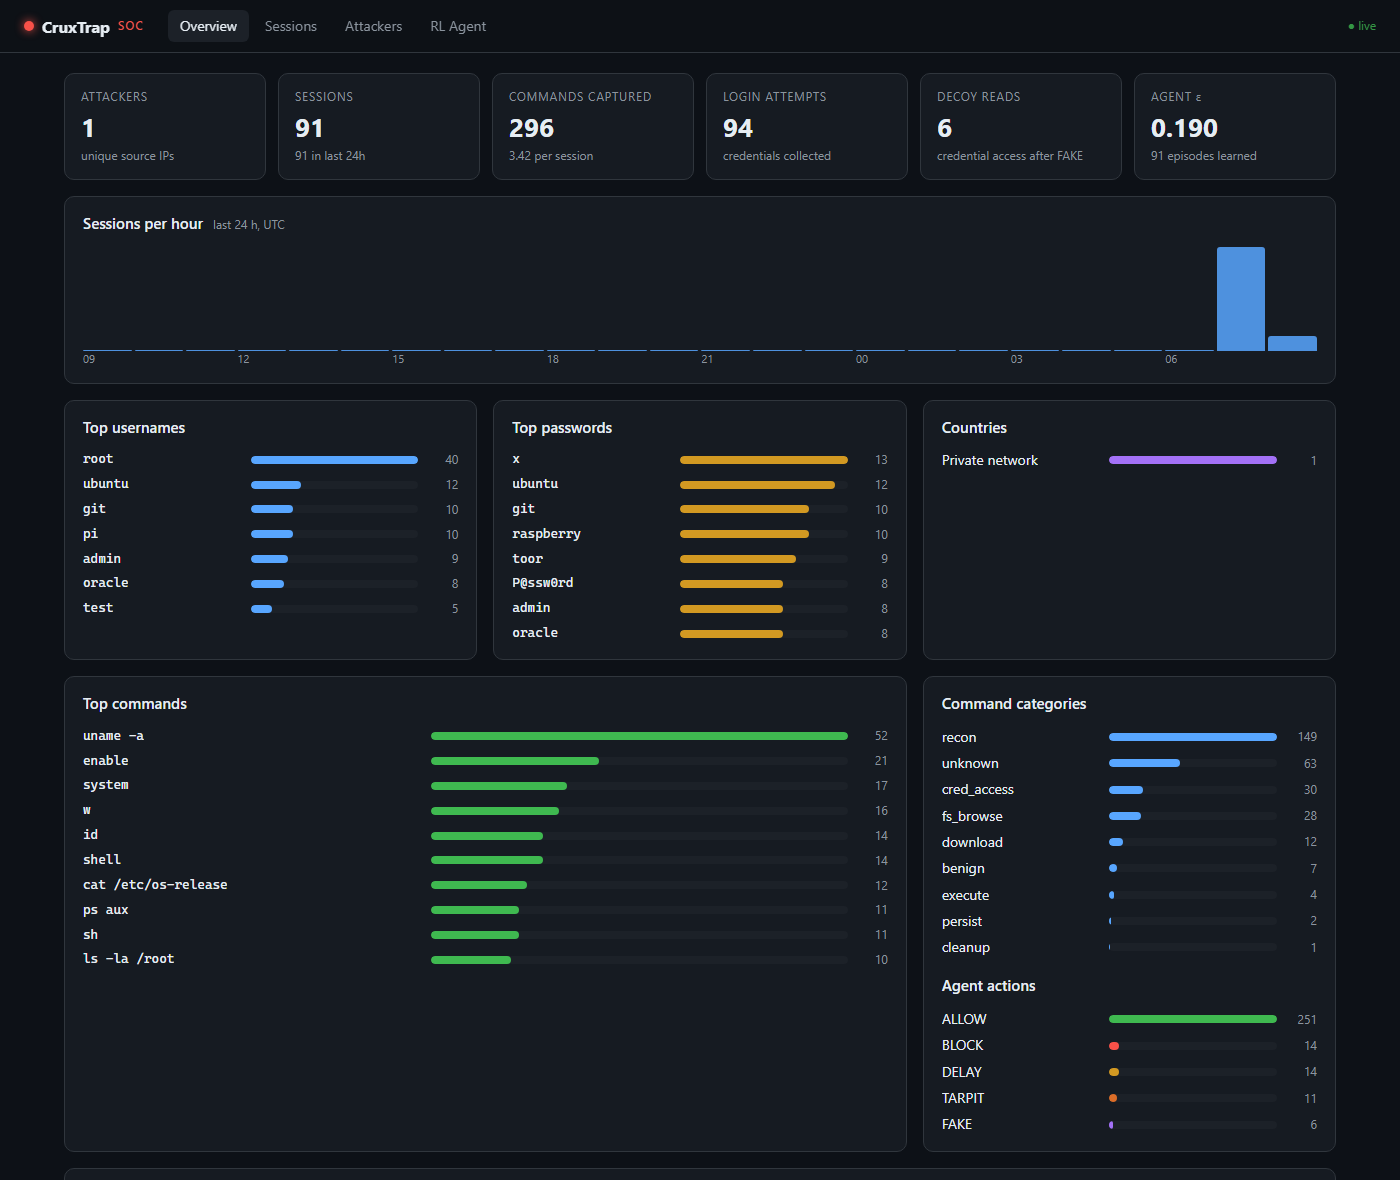
\includegraphics[width=\textwidth]{shot_overview.png}
\caption{Dashboard overview (lab-generated traffic).}
\label{fig:shot-overview}
\end{figure}

\begin{figure}[H]
\centering
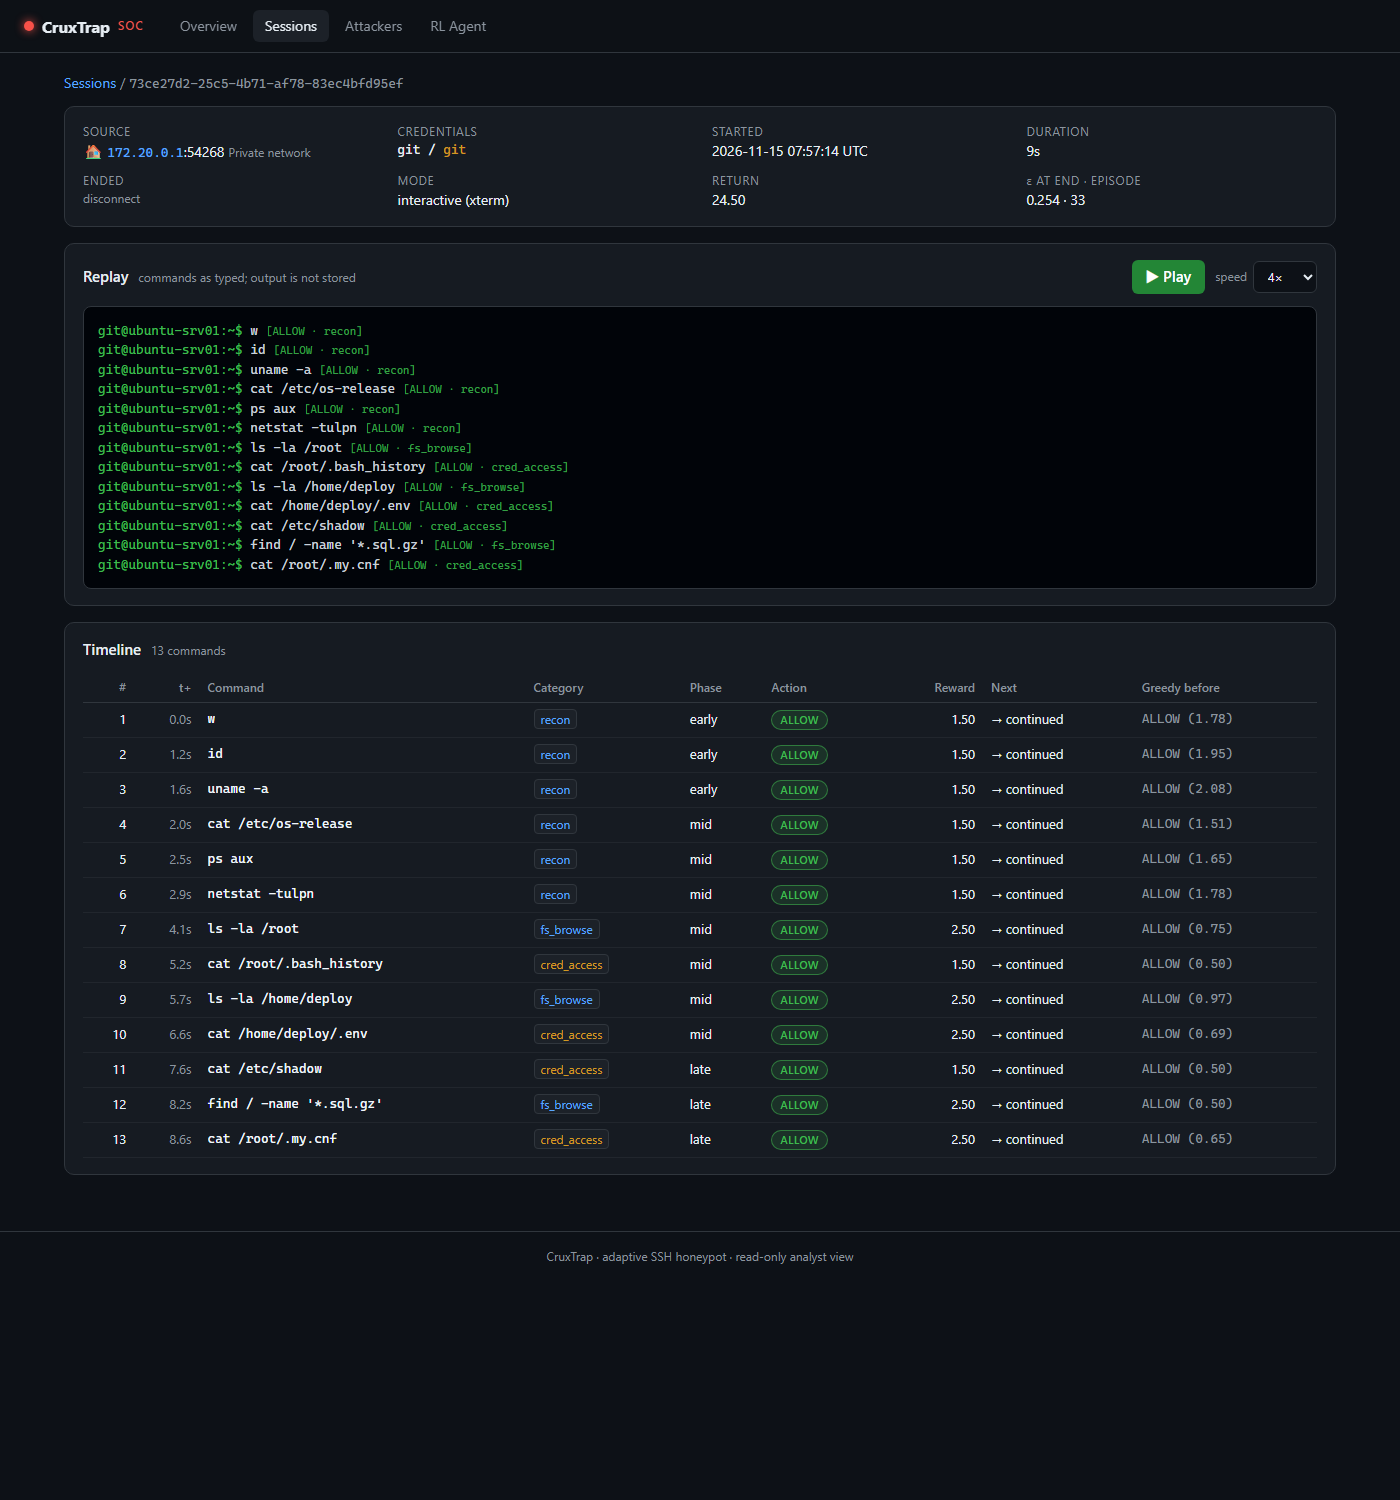
\includegraphics[width=\textwidth]{shot_session.png}
\caption{Session detail: terminal replay and per-command timeline with the agent's decisions.}
\label{fig:shot-session}
\end{figure}

\begin{figure}[H]
\centering
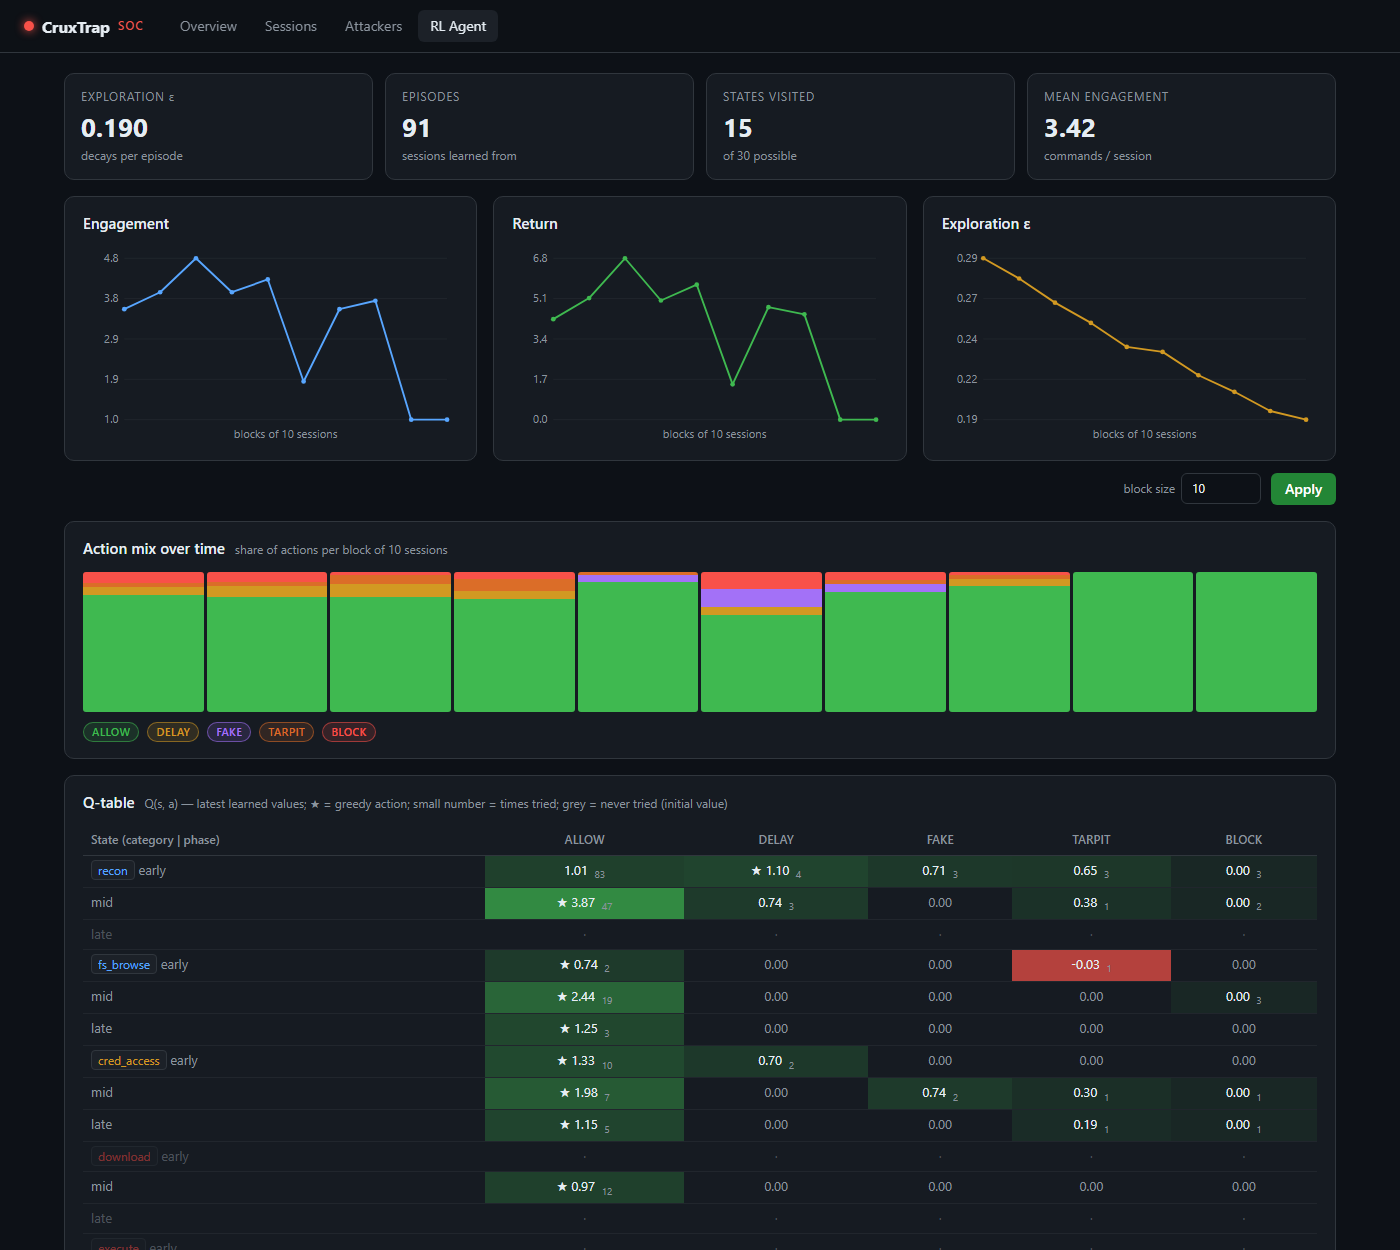
\includegraphics[width=\textwidth]{shot_rl.png}
\caption{RL view: learning curves, action mix over time and the Q-table heatmap.}
\label{fig:shot-rl}
\end{figure}

\section{Deployment}

Each Python service has its own image based on \code{python:3.12-slim} and runs as an
unprivileged user (UID 10001). Docker Compose defines the five services, their health checks,
start-up order (dependent services wait for healthy dependencies), three named volumes
(database, Redis append-only file, and honeypot keys plus Q-table), and two networks
(Figure~\ref{fig:arch}). Every published port binds to \code{127.0.0.1} by default. A real
deployment exposes only the honeypot, typically on port 22 after moving the host's own SSH
daemon. Table~\ref{tab:hardening} lists the hardening of the honeypot container.

\begin{table}[H]
\centering
\small
\begin{tabularx}{\textwidth}{@{}lX@{}}
\toprule
\textbf{Layer} & \textbf{Measure} \\
\midrule
Application & Emulation only: no \code{exec}, \code{subprocess} or shell anywhere in the command path \\
Process & Non-root UID 10001; effective capability set empty (\code{cap\_drop: ALL}); \code{no-new-privileges} \\
Filesystem & Read-only root filesystem; 16\,MB \code{tmpfs} at \code{/tmp} \\
Resources & 256 processes, 512\,MB memory, 1 CPU \\
Network & \code{ingest} network only: Redis reachable, PostgreSQL not resolvable \\
Health check & Reads \code{/proc/net/tcp} for the listening socket instead of connecting, so health probes are not recorded as attackers \\
\bottomrule
\end{tabularx}
\caption{Hardening of the internet-facing container.}
\label{tab:hardening}
\end{table}

\paragraph{Source addresses.} On Docker Desktop (Windows and macOS), published ports pass
through a user-space proxy, and the honeypot sees every client as the Docker gateway address.
On a Linux host, connections from the Internet are forwarded by iptables DNAT and keep their
real source address. The honeypot must therefore be deployed on Linux, or with host
networking, for the source-IP telemetry to be meaningful.
